\documentclass{article}

\usepackage{pgfplots}

\pgfplotsset{compat=1.16}

\begin{document}

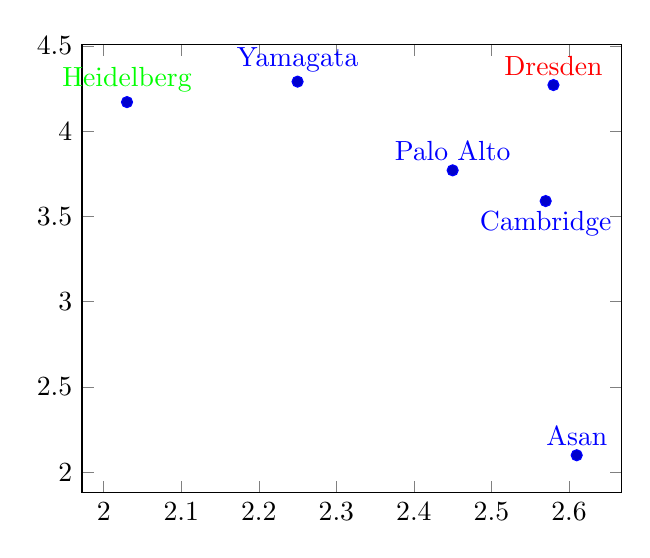
\begin{tikzpicture}
	\begin{axis}
		\addplot+ [
			nodes near coords,
			only marks,
			coordinate style/.condition={\coordindex==0}{below},
			coordinate style/.condition={\coordindex==1}{red},
			coordinate style/.condition={y > 4 && x < 2.1}{green},
			point meta=explicit symbolic,
		] table [meta=label] {
			Depth Breadth label
			2.57 3.59 Cambridge
			2.58 4.27 Dresden
			2.45 3.77 {Palo Alto}
			2.61 2.10 Asan
			2.03 4.17 Heidelberg
			2.25 4.29 Yamagata
		};
	\end{axis}
\end{tikzpicture}

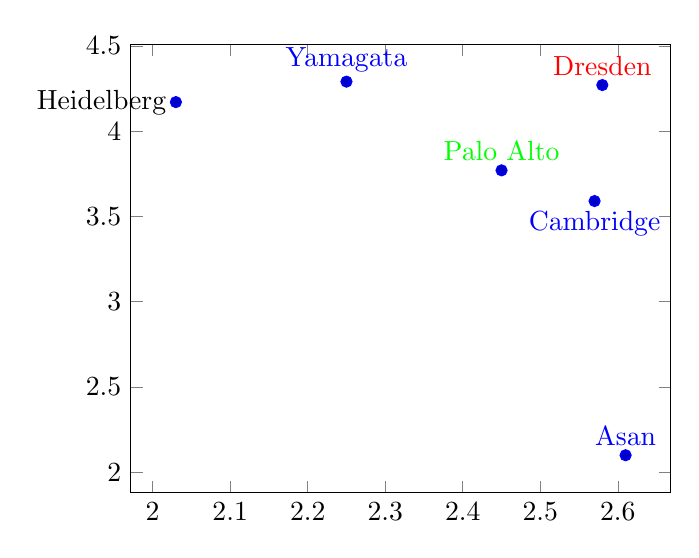
\begin{tikzpicture}
	\begin{axis}
		\addplot+ [
			nodes near coords,
			only marks,
			coordinate style/.from=\thisrow{style},
			coordinate style/.condition={y > 4 && x < 2.1}{black},
			point meta=explicit symbolic,
		] table [meta=label] {
			Depth Breadth label style
			2.57 3.59 Cambridge below
			2.58 4.27 Dresden red
			2.45 3.77 {Palo Alto} green
			2.61 2.10 Asan {}
			2.03 4.17 Heidelberg {left}
			2.25 4.29 Yamagata {}
		};
	\end{axis}
\end{tikzpicture}
\end{document}

